\section{Magnetooptischer Kerr-Effekt}

\subsection{Theoretische Grundlagen}

  \subsubsection{Magnetisierung von Materie}

  Äußere Magnetfelder $\vec{H}$ verusachen in Materie eine materialabhängige makroskopische Magnetisierung $\vec{M}$.
  In dia- ($\chi_V<0$) und paramagnetischen ($\chi_V>0$) Materialien lässt sich dieser Zusammenhang mit der Vakuumpermeabilität $\mu_0$ durch
  \begin{equation}
    \mu_0 \vec{M} = \chi_V \vec{B}_0
  \end{equation}
  beschreiben.
  Die Magnetisierung hängt also über $\chi_V$ linear von der äußeren magnetischen Flussdichte $\vec{B}_0= \mu_0 \vec{H}$ ab.

  In ferromagnetischen Materialien hingegen bleibt nach Abschalten des äußeren Magnetfeldes eine Magnetisierung zurück, die zu der in \cref{fig_magnetismen} abgebildeten Hysteresekurve führt.

  \begin{figure}[H]
      \centering
      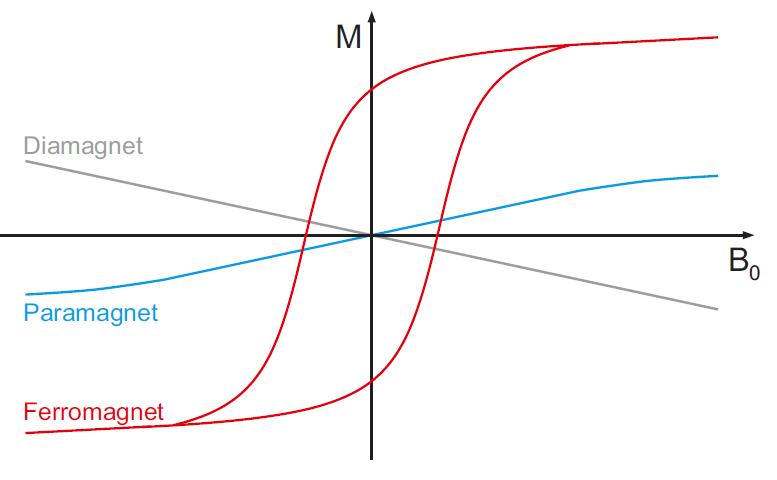
\includegraphics[width=0.8\textwidth]{img/magnetismen}
      \caption{Schematische Abhängigkeit der Magnetisierung $M$ dia-, para- und ferromagnetischer Materialien vom angelegten äußeren Magnetfeld $B$. \cite{anleitung}}
      \label{fig_magnetismen}
  \end{figure}

  %den Kram mit den Domänen lasse ich jetzt weg, weils irgendwie weitgehend egal ist.

  \subsubsection{Polarisation und Materie}
  Die Wechselwirkung von elektromagnetischen Wellen mit Materie kann über den komplexen Brechungsindex
	\begin{align*}
		\tilde{n} = n + ik
	\end{align*}
  mit der Brechung $n$ und der Absorption $k$ beschrieben werden.
  Hieraus kann Reflektion und Transmission berechnet werden.
  Das Hinzufügen eines externen magnetischen Feldes verursacht wie beschrieben eine Magnetisierung in Abhängigkeit von den magnetischen Eigenschaften der Materie.
  Dadurch ändert sich auch der Brechungsindex je nach Polarisation der einfallenden elektromagnetischen Welle.

  Linear polarisiertes Licht kann als Überlagerung einer rechts- und einer linkszirkular polarisierten elektromagnetischen Welle beschrieben werden.
  Beim Treffen auf Materie werden diese Teilwellen mit unterschiedlicher Intensität und Phase reflektiert bzw. transmittiert.
	Im Ergebnis ist die Überlagerung der Wellen nicht mehr linear, sondern elliptisch polarisiert.
	Die Winkeldifferenz zwischen Hauptachse der Ellipse und der Polarisationsrichtung des initialen linear polarisierten Lichts ist die Rotation und die Änderung der Intensität ist die Exzentrizität.

  Die Rotation wird im Falle von Transmission Faraday-Rotation und im Falle von Reflektion Kerr-Rotation mit dem Kerr-Winkel $\theta_K$ genannt.

  In Ferromagneten liegen stets unterschiedlich magnetisierte Domänen (weissche Bezirke) vor.
  Da jedoch bei Messungen des Kerr-Winkels viele Domänen belichtet werden, wird ein mittlerer Kerr-Winkel gemessen, der als proportional zur Magnetisierung angenommen werden kann.

\subsection{Aufbau \& Durchführung}

  \begin{figure}[H]
      \centering
      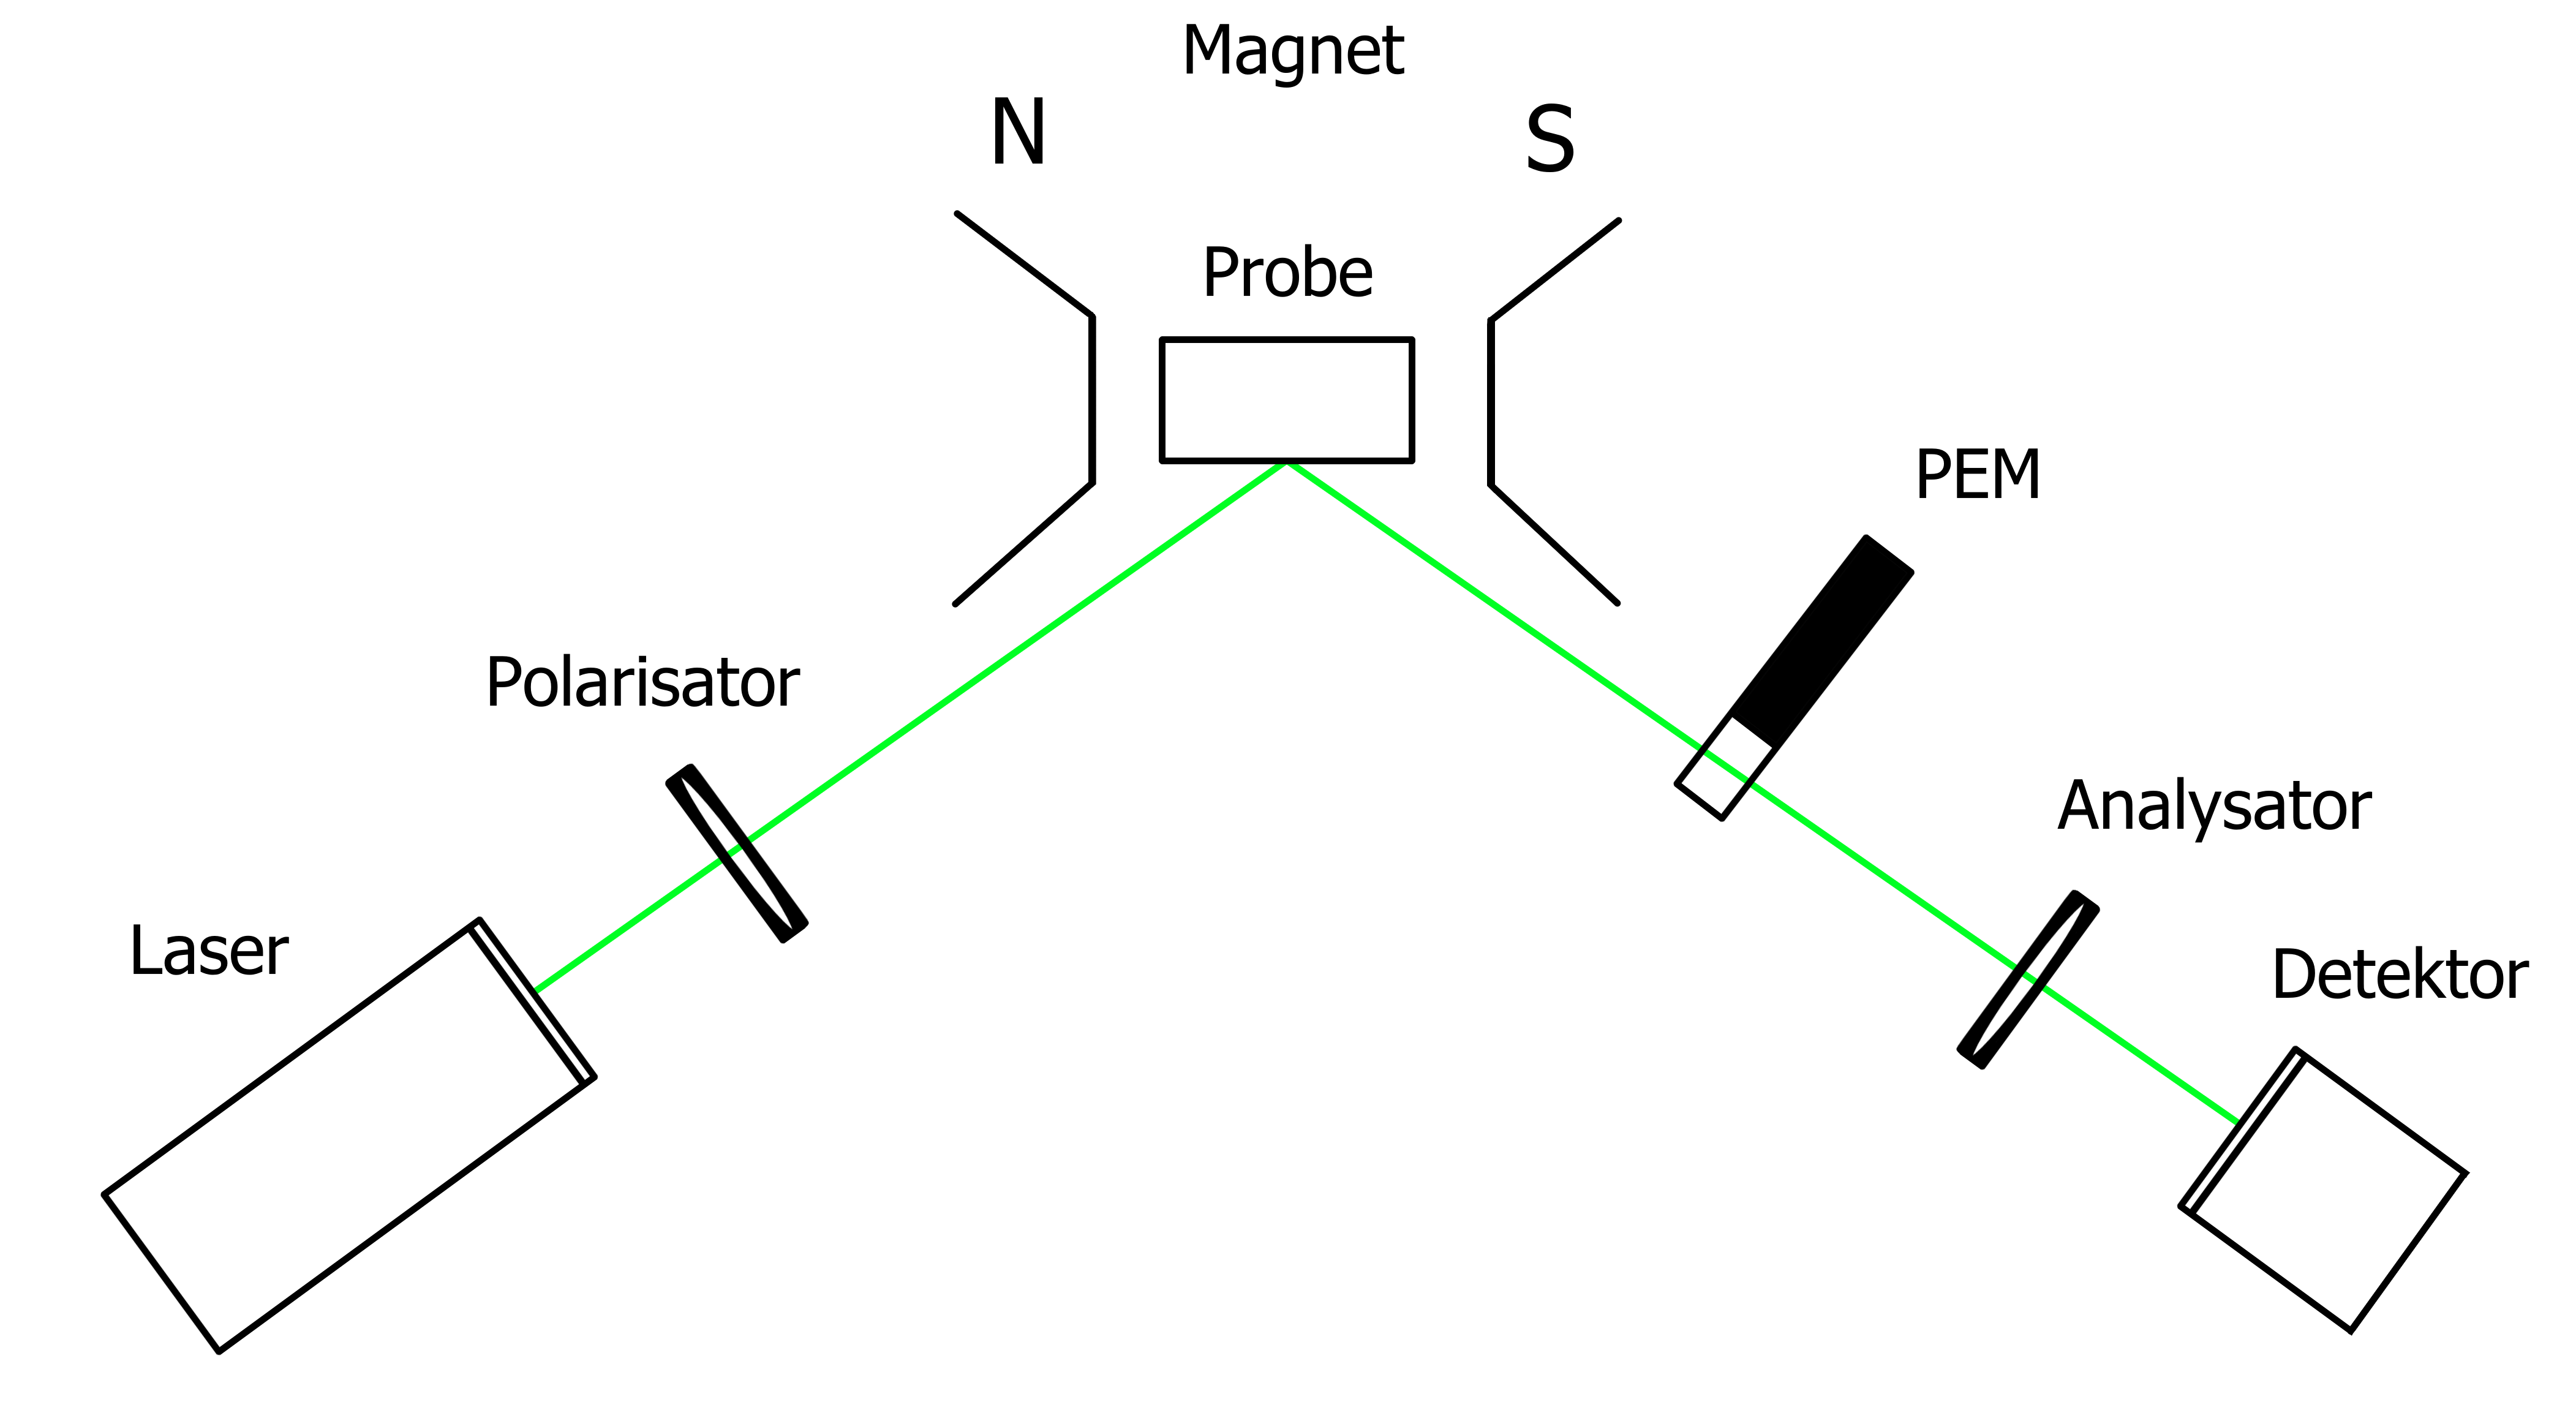
\includegraphics[width=0.8\textwidth]{img/setup2}
      \caption{Schematische Darstellung des experimentellen Aufbaus zur Messung der Magnetisierung in Abhängigkeit vom äußeren Magnetfeld. Abgebildet ist die Konfiguration zur Messung des magnetooptischen Kerr-Effekts in longitudinaler Richtung. Die Polschuhe des Elektromegneten können in der Zeichenebene um \SI{90}{\degree} gedreht werden, um in polarer Richtung messen zu können. PEM steht für photoelastischer Modulator. Die Polarisatoren sind Glan-Thompson-Prismen.}
      \label{fig_setup2}
  \end{figure}

  In \cref{fig_setup2} ist der experimentelle Aufbau dargestellt, der verwendet wird, um die Magnetisierung in Abhängigkeit von einem äußeren Magnetfeld sichtbar zu machen.
  Durch Drehen des Elektromegneten kann die Ausrichtung des Magnetfelds relativ zur Ebene und Einfallsrichtung geändert werden, sodass in longitudinaler oder polarer Richtung gemessen werden kann.

  Zur Kalibration wird als Probe ein Spiegel verwendet, mit dem die optischen Elemente so ausgerichtet werden, dass das gemessene Signal maximiert wird.
  Um möglichst empfindlich gegenüber Änderungen der Polarisation zu sein, wird der Analysator in einen \SI{45}{\degree}-Winkel zum Polarisator gebracht, indem der Mittelpunkt zwischen maximaler und minimaler Transmission eingestellt wird.
  Dadurch bewegt sich die Polarisation auf der Flanke der Sinuskurve des Gesetzes von Malus, sodass kleine Änderungen in der Polarisation zu einer maximalen Änderung der Intensität führen.
  Außerdem kann die Sinuskurve hier als linear genähert werden, sodass eine Proportionalität zwischen Intensitätsänderung und Polarisationsänderung besteht.

  Dann wird eine Kalibrationsmessung für das Magnetfeld durchgeführt, indem eine Hall-Sonde an die Stelle der Probe gebracht wird und der Spulenstrom schrittweise erhöht wird.
  Es wird ein photoelastischer Modulator verwendet, um dem reflektierten Laserstrahl eine Modulation hinzuzufügen, die in Kombination mit einem Lock-In-Verstärker eine erhöhte Messgenauigkeit erlaubt.
  Da lediglich über die Intensität auf den Kerr-Winkel und über diesen auf die Magnetisierung geschlossen wird, ist es nur möglich, die Magnetisierung in willkürlichen Einheiten anzugeben.

  Es werden je 10 Messkurven für eine CoPt-Probe und eine CrO$_2$-Probe aufgenommen, indem der Spulenstrom graduell erhöht und wieder gesenkt wird, sodass die Hysteresekurve gemessen wird.
  Sollte sich schnell herausstellen, dass die Probe in einer Magnetfeldausrichtung nicht magnetisierbar ist, wird keine vollständige Messung durchgeführt. %er meinte, in der Richtung nicht magnetisierbar. Das hieße ja, dass das Einkristalle sind. Man könnte halt auch behaupten, dass einfach in der Richtung kein moke, aber trotzdem Magnetisierung stattfindet.


\subsection{Ergebnisse \& Diskussion}

%CoPt ist nur Out of plane Magnetisierbar. Der CrO2 nur in plane. Die jeweils anderen nur kurz gemessen, um das festzustellen.
CoPt ist nur in der polaren Messung magnetisierbar und CrO$_2$ nur in der longitudinalen Messung.
Die Unsicherheit der Magnetisierung wird auf Basis der Streuung der Daten bei im Betrag hohen Magnetfeldstärken abgeschätzt, da hier die Magnetisierung konstant sein sollte.
Die Unsicherheit der Magnetfeldstärke wird als demgegenüber vernachlässigbar angenommen.

\begin{figure}[H]
    \centering
    \begin{subfigure}{0.465\textwidth}
        \centering
        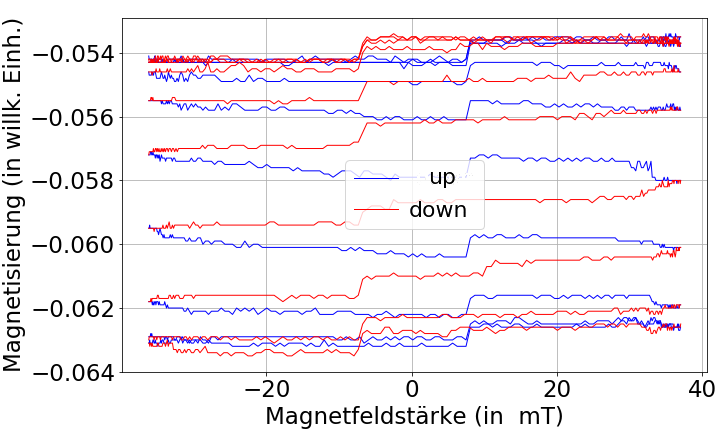
\includegraphics[width=1.1\textwidth]{plots/swp_cro_raw}
    \caption{CrO$_2$}
    \end{subfigure}
    \hfill
    \begin{subfigure}{0.465\textwidth}
        \centering
        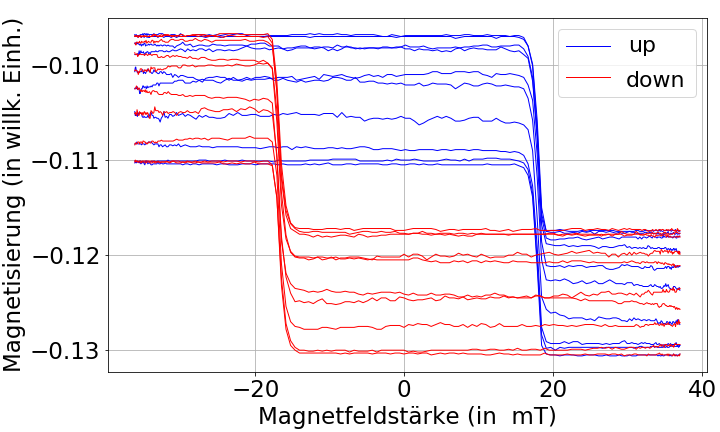
\includegraphics[width=1.1\textwidth]{plots/swp_copt_raw}
        \caption{CoPt}
    \end{subfigure}
    \caption{Unbearbeitete Messdaten beider Proben. \enquote{up} steht für steigende und \enquote{down} für fallende Magnetfeldstärke. Die Unsicherheiten wurden zugunsten der Übersicht nicht dargestellt.}
      \label{fig_moke_raw}
\end{figure}

  In \cref{fig_moke_raw} ist das Ergebnis der Messungen dargestellt.
  Es ist deutlich sichtbar, dass während der Messung ein thermischer Drift stattfindet, der die gemessene Intensität über die Messungen wandern lässt.
  Da die Magnetisierbarkeit (die Aufspaltung zwischen positiver und negativer Magnetisierung) der CrO$_2$-Probe deutlich größer ist, fällt dies hier stärker ins Gewicht.
  Um dies zu korrigieren werden zunächst alle Messungen über ihren Mittelwert so angepasst, dass die durchschnittliche Intensität der Messungen (für auf- und absteigende Messungen einzeln) etwa konstant ist.
  Zusätzlich wird ein konstanter thermischer Drift innerhalb der Messungen angenommen und die Messungen so korrigiert, dass die Kurven bei im Betrag sehr hohen Magnetfeldern konstant sind.
  Dies ist in \cref{fig_moke_einzeln} abgebildet.
  Hier wird auch sichtbar, dass die geringe Präzision der Gleitkommazahlen im Messergebnis bei der CrO$_2$-Probe aufgrund der geringen Magnetisierbarkeit zu Rundungsfehlern führt. %Genius...

\begin{figure}[H]
    \centering
    \begin{subfigure}{0.495\textwidth}
        \centering
        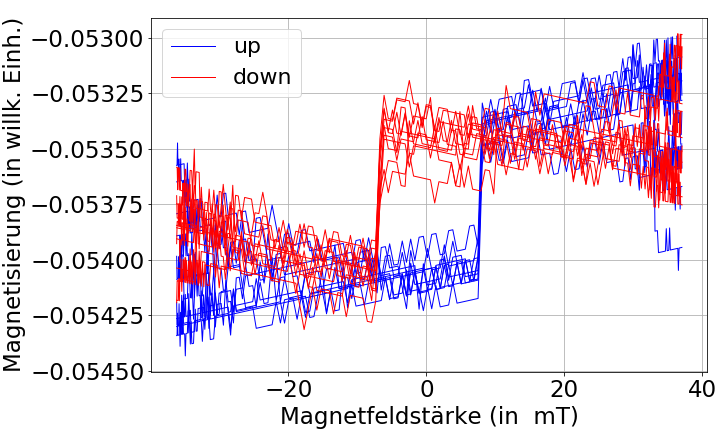
\includegraphics[width=1.1\textwidth]{plots/swp_all_magn_cro}
    \caption{CrO$_2$}
    \end{subfigure}
    \begin{subfigure}{0.495\textwidth}
        \centering
        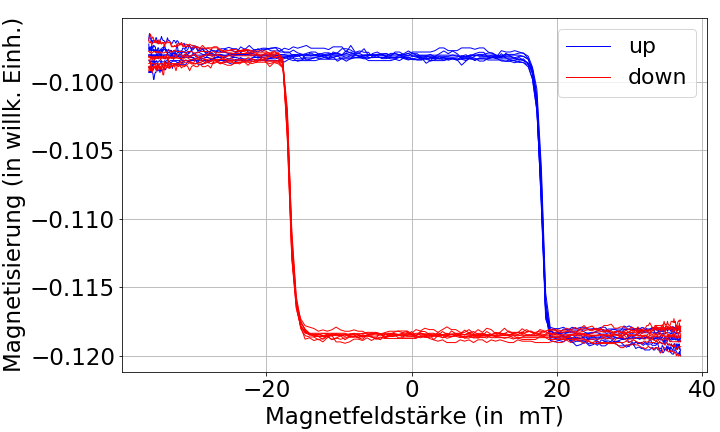
\includegraphics[width=1.1\textwidth]{plots/swp_all_magn_copt}
        \caption{CoPt}
    \end{subfigure}
    \caption{Um den thermischen Drift korrigierte Messungen der Hysteresekurven von CrO$_2$ und CoPt. \enquote{up} steht für steigende und \enquote{down} für fallende Magnetfeldstärke. Die Unsicherheiten wurden zugunsten der Übersicht nicht dargestellt.}
    \label{fig_moke_einzeln}
\end{figure}

Aus diesen zehn Messungen werden nun jeweils Mittelwerte gebildet und in \cref{fig_moke_averages} dargestellt.
Es ist bei beiden Messungen deutlich die Hysterese zu erkennen, wobei im Falle der CoPt-Probe die Magnetisierbarkeit deutlich höher ist.


\begin{figure}[H]
    \centering
    \begin{subfigure}{0.495\textwidth}
        \centering
        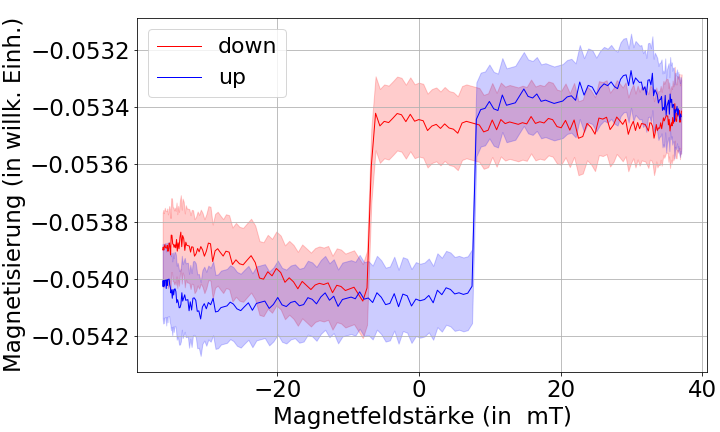
\includegraphics[width=1.1\textwidth]{plots/swp_avg_magn_man_cro}
    \caption{CrO$_2$}
    \end{subfigure}
    \begin{subfigure}{0.495\textwidth}
        \centering
        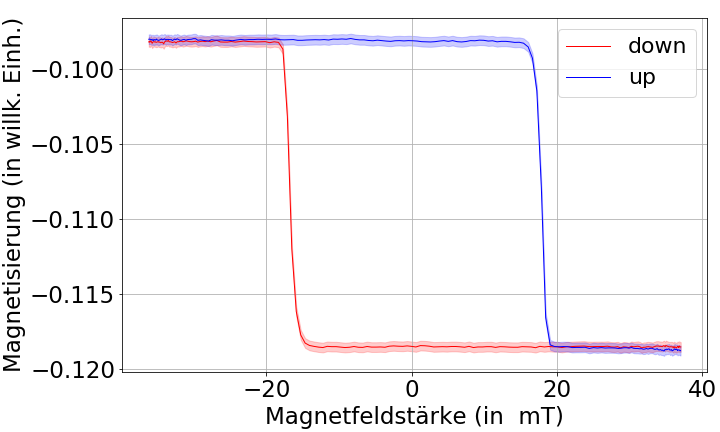
\includegraphics[width=1.1\textwidth]{plots/swp_avg_magn_man_copt}
        \caption{CoPt}
    \end{subfigure}
    \caption{Gegen den thermischen Drift korrigierte gemittelte Messungen der Hysteresekurven von CrO$_2$ und CoPt. \enquote{up} steht für steigende und \enquote{down} für fallende Magnetfeldstärke.}
    \label{fig_moke_averages}
\end{figure}
